\section{Dataset 1: Diabetes Dataset (Regression)}

\subsection{ANFIS}

Continuing on assignment 1's work, the model was trained with ANFIS method. The training parameters were tuned with a grid search method culminating in the best values of:

n\_iterations: 3
gd\_epochs: 10
lr: 0.01

With these parameters the resulting model had an ACC of 0.8206896551724138.

\begin{figure}[h!]
    \centering
    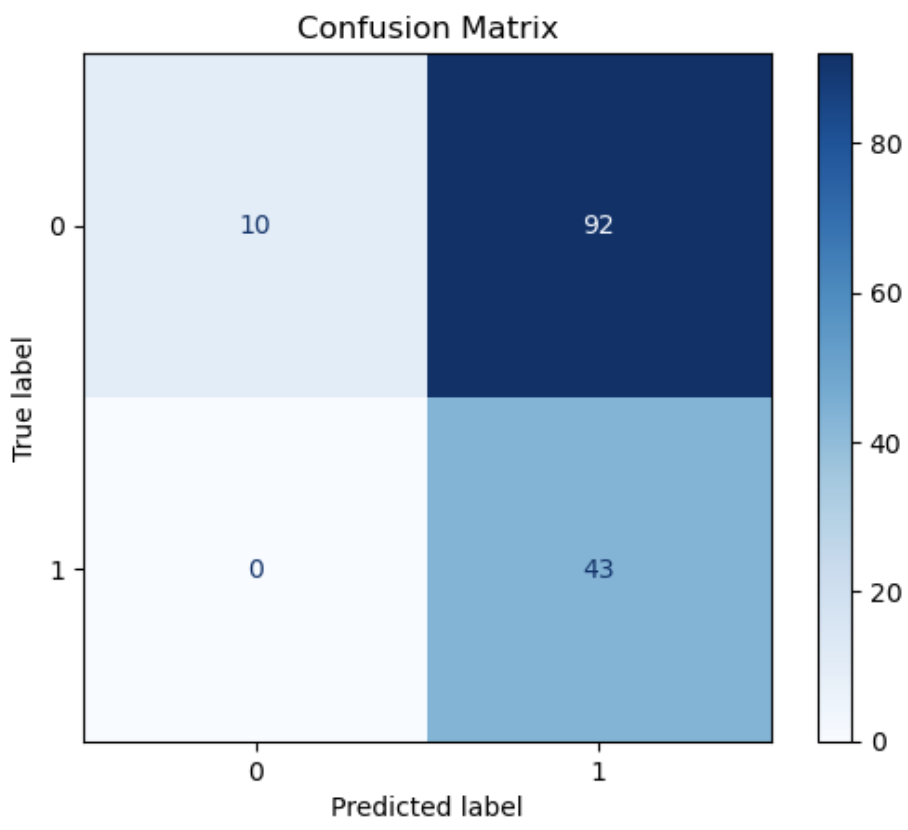
\includegraphics[width=0.5\textwidth]{Plots/ConfusionMatrixANFIS.png}
    \caption{Confusion Matrix}
    \label{fig:my_label}
\end{figure}

\begin{figure}[h!]
    \centering
    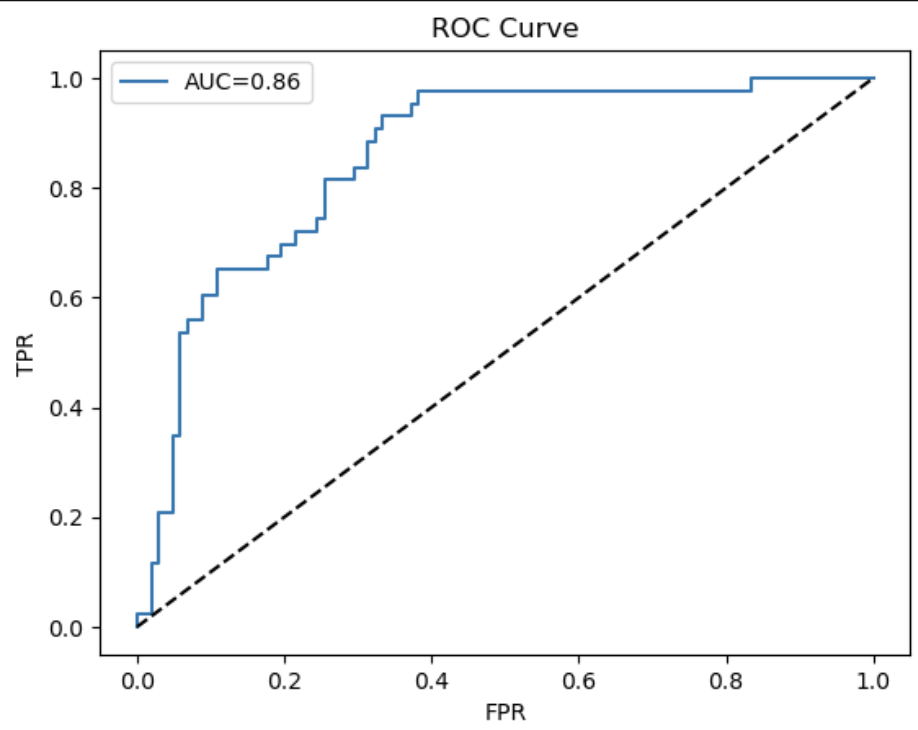
\includegraphics[width=0.5\textwidth]{Plots/RoCANFIS.png}
    \caption{ROC}
    \label{fig:my_label}
\end{figure}

\subsection{MLP}

For the MLP, the parameters where manually tuned:

num\_epochs=100
lr=0.0003
dropout=0.2
batch\_size=64

Testing different neural network layer configurations wasn't done.

The resulting model had an ACC of 0.7931034482758621.

\begin{figure}[h!]
    \centering
    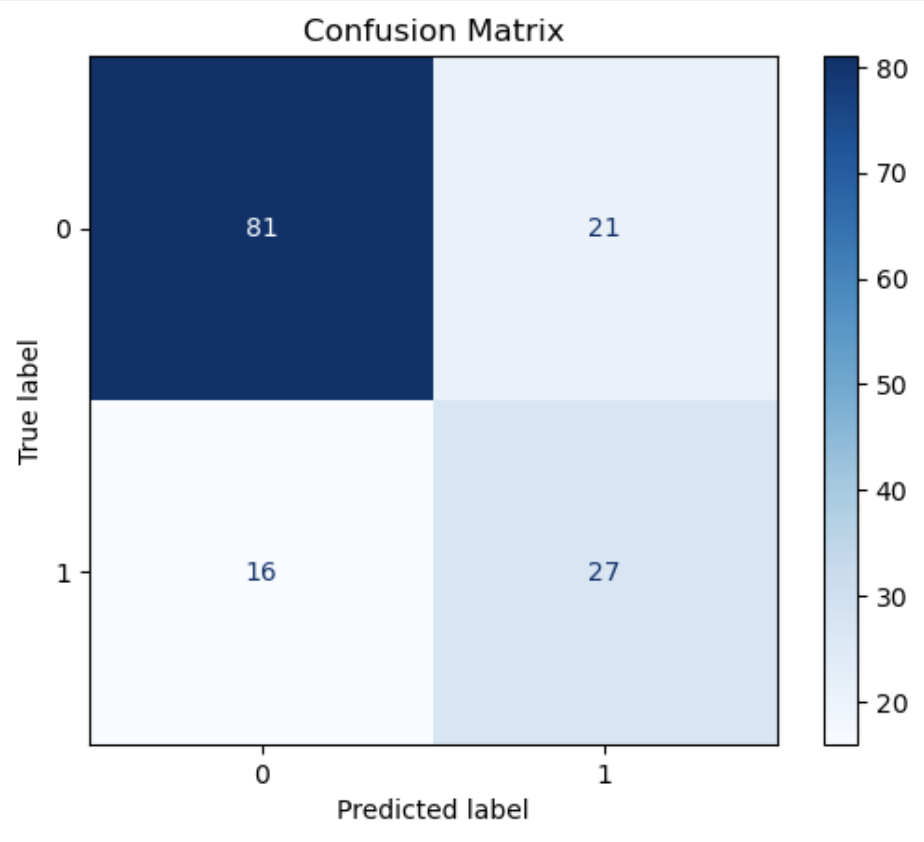
\includegraphics[width=0.5\textwidth]{Plots/ConfusionMatrixMLP.png}
    \caption{Confusion Matrix}
    \label{fig:my_label}
\end{figure}

\begin{figure}[h!]
    \centering
    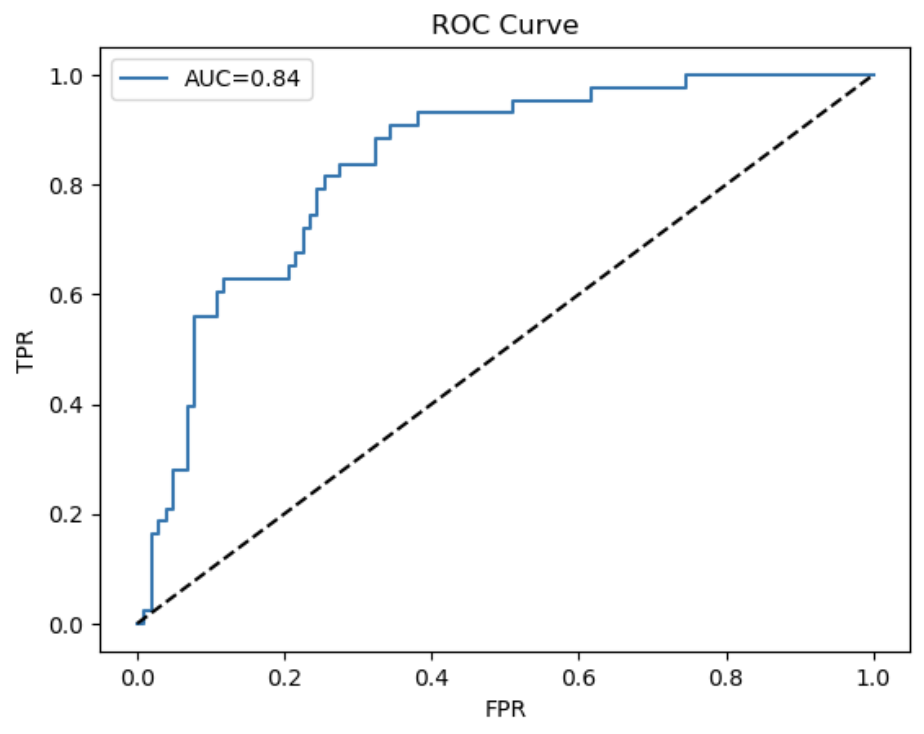
\includegraphics[width=0.5\textwidth]{Plots/RoCMLP.png}
    \caption{ROC}
    \label{fig:my_label}
\end{figure}

